\chapter{Results}
\label{ch:results}

The qualitative results fall into three parts.
%
First, personal reflections on my approach to interviews and drawing
from Indigenous knowledge - and how I underestimated the complexity
of seasonal calendars.
%
Second, commentary on how to accurately characterise Yonlgu seasons.
This section covers required datasets, historical changes, spatial
variation in definitions, and three distinct types of season.
%
Third, a Yolngu seaonal calendar drawn from interview responses,
defining a handful of meteorologically-defined seasons each year.

The quantitative results follow, starting with a summary of the
observational weather record.  Finally, the quantified seasons are
presented.



\section{Unexpected Complexity in Seasonal Calendars}
\label{sec:complex-seasons}



\subsection{Reflection - Complex Calendars as an emergent theme}

`Calendar' and `season' are not concepts that translate directly across cultures.

Discuss how I realised this, by re-listening to recordings, and that I was
expecting something unforeseen (but not like this!).

Note that informal, collaborative and participant-led conversations were key.

\todo{expand points to paragraphs, with quotes}

\begin{itemize}
\item all in english
\item what is a season
\item what is a calendar
\item there is no ``the'' yolngu calendar - varies spatially,
        multiple seasonal calendars for different temporal scales with varied purposes
\item `simple fact-finding' really isn't!
\item unusual or extreme events people remember, and how these fit into the calendar
\item understandings of climate change including expected impacts (minimal, after \citet{petheram2010})
\end{itemize}



\subsection{Yolngu Seasons vary by location and temporal scale}
\label{subsec:three-seasons-scales}

Yolngu participants discussed seasons at three distinct temporal scales
each year, each type recognised by different indicators.
\begin{itemize}
\item `Monsoon seasons' - Wet and Dry - are recognised not by rainfall but
        by winds from the north-west and south-east respectively.
\item The six `weather seasons' are defined primarily by wind, rain, and temperature.
        They can begin and end at any time during the year - weather permitting -
        and may occur more than once and in any order.
\item Complex `ecological seasons', where changes in plant or animal life
        signal appropriate activities for that time.  A particular community
        may recognise tens of these, all highly localised.
\end{itemize}

This three-level typology emerged from interview data, prompted by
the patterns in timescale and kinds of indicators for each.
While it forms a more nuanced view than disregarding all but a single or
simplified seasonal calendar, this too falls far short of the richness
and detail of Yolngu understandings.
%
Ian Morris, who was a teacher at the Galiwinku mission for many years,
said \blockquote{
    QUOTE IAN RE: could not possibly fit everything on a wall
}

A similar three-level pattern of seasons is visible in \cref{fig:tiwi-seasons},
on page~\pageref{fig:tiwi-seasons}.  The Tiwi seasons are shown at a monsoonal level,
as well as by weather or ecology.  The latter categories are not clearly distinguished
in this figure, though weather is generally further from the center.


\subsubsection{Monsoon Seasons (Wet/Dry)}

Each year, there is a wet season and a dry season.  These seasons are
recognised by the monsoon winds from the north-west and south-east
respectively.  Some years have a gap-filling season between them.

Of the three levels of seasons recognised by Yolngu,
the wet/dry monsoon seasonal cycle is most likely familiar to non-Indigenous people -
especially in the tropics.  Yolngu participants emphasised that these seasons
are \emph{not} recognised by rainfall, but rather the direction of prevailing winds.

\blockquote{
    ADD QUOTE HERE - RR.
}

Interestingly, this mirrors the meteorological definition of monsoon,
where rainfall is less important than the location of the intertropical
convergence zone and consequent direction of prevailing wind.
This shared understanding of monsoon seasonality should not go unremarked -
but does direct this research to the more local seasonal patterns.


\subsubsection{Meteorological Seasons}

At the middle timescale, Yolngu recognise six seasons.
The Wet season is divided into \textit{Dhuludur}, \textit{Barramirri},
and \textit{Mayaltha}, followed by \textit{Midawarr}, \textit{Dharrathamirri},
and \textit{Rarrandharr} over the Dry.  Detailed descriptions of each
season from interviews, supported by literature extracts, can be found below.
%
These seasons are primarily defined by weather conditions and events,
which are shared across communities in the area.  Ecological indicators
also play a role in recognising meterological seasons, which people
\textit{mangutji bulthanaway} (``possessing the quality of telling the eye'')
can interpret \citep[p35]{atlas2014}.  The distinction from ecological
seasons is supported by local differences in indicators, but ultimately
derives from limitations in the scope of this research rather than
Yolngu understanding.

Quantification and analysis focusses on meteorological seasons.
Data availability is one reason:  the installation of automatic weather
stations at Arnhem Land airports in the 1990s and early 2000s provide
and new but solid daily observational record of many weather variables.
By contrast the Monsoon has been the subject of many studies, while
detailed ecological or phenological records at the required temporal
resolution are very rare.

Meteorological seasons also match up reasonably well with mainstream --
that is, European-derived -- ideas of what a season should be.  Wet/Dry
is well-known but permits little nuance, while ecological seasons are
alienatingly complex and detailed.  Six per year and defined by weather
is not \emph{too} exotic for productive collaboration across varied
ideas of what seasons are like!
%
However, there are also critical differences that are too rarely shown.

\todo{outline variability in timing, WITH QUOTES, multiple-onset, etc.
This is where the claims get backed up with data!}






\subsubsection{Ecological Seasons}
Ecological seasons are defined by observed changes in local vegetation
and animal behaviour.  They embody a depth and detail of Indigenous
ecological knowledge that is difficult to imagine, and only possible
due to the long connection between Yolngu and the natural environment.

Participants explained that these seasons vary between groups even within
a single clan-nation or language group, meaning that each of the towns
across Arnhem Land (see \cref{fig:arnhem-map}) would have a different
calendar. These seasons are closely tied to traditional activities such as
travel, use of particular foods or other resources, and ceremony.

On the Tiwi Seasons Calendar, \cref{fig:tiwi-seasons}, the inner-most
rings concern ecological seasons and observations - such as
\textit{Mumpikari}, when possums leave muddy tracks and hunting them is easy.

However, certain practicalities put ecological seasons beyond scope
for the remainder of this thesis.
The same detail and diversity which makes these seasons so fascinating
also mandates far greater investment of time and travel to speak
with the relevant knowledge holders, and proper study would require
living in each community for a significant period.
Sensitive, sacred, or unpublishable stories and information are much more
common around ecological seasons than the more general calendar,
and researchers have obligations in this area which are not always clear.
Generalisation between communities is difficult if not impossible.
And finally, quantification would be very difficult due to the paucity
of quantitative ecological data at the required level of detail
and localisation, especially in `remote' Australia.

\Cref{sec:further-study} discusses how these seasons might be explored
by further research, and some of the challenges to overcome.



\subsection{Other Advice on Detecting Seasons}
\label{subsec:detection-advice}
Yolngu participants made several comments which are not about
the seasonal calendar itself, but are of vital importance when quantifying
it - teaching about how exactly to recognise each season.

\begin{description}
\item[Variation between years]
    Yolngu seasons vary between years, depending on the weather conditions.
    Participants said that the seasons had always been steady within this
    normal variation.  When asked about climate change, participants were
    concerned about environmental changes and attributed many to human
    activity - including mining, but also loss of traditional knowledge
    and respect for the land.

\item[Unordered or duplicated seasons]
    Seasons are not limited to a particular order, and may happen one or more
    times per year (by definition zero or more; historically at least once).
    Any season may be `interrupted' by another if the latter's characteristic
    conditions hold.  It is important to avoid hasty judgement however, so this
    takes at least two or three days of atypical weather.

    Where non-indigenous people might discuss a `cold snap', Yolngu might
    say that winter had interrupted summer!

\item[Wind and the sea breeze]
    Wind plays a defining role in Yolngu seasons, but not all winds are
    seasonal indicators.  In coastal communities, the day-time and especially
    afternoon wind is dominated by the sea breeze, and carries relatively little
    seasonal information.

    Participants said that morning wind at 9am would be fine, but that at
    3pm the sea breeze overwhelms the seasonal changes.  The suggestion was
    to instead consider wind between 5pm and 8pm depending on time of year.

    With data at three-hourly resolution, \cref{fig:galiwinku-seabreeze-direction}
    does not show a substantially stronger seasonal signal at 6pm than 3pm.
    I therefore use the standard observations of 9am and 3pm for the analysis.

\end{description}



\section{A Qualitative Yolngu Seasonal Calendar}
\label{sec:calendar-description}

The remainder of this thesis focusses on a six-season Yolnu calendar with
meteorological definitions.  It is based primarily on interview data, within
the framework provided by \textit{Man of All Seasons} \citep{davis1989} and
\textit{Yan-nhangu Atlas} \citep{atlas2014} -- recognising that all of these
sources describe different communities and areas.  When sources conflict, I
use participant comments from Galiwinku.

Readers should note that this is not a definitive Yolngu calendar; no such
thing exists.  Instead it represents my attempt to construct a quantifiable
Yolngu seasonal calendar from as many sources as possible, and show some of
the challenges of working with complex, incomplete, and sometimes missing
information.  I am confident that the result is fit for purpose, and -- taken
with \cref{sec:complex-seasons} -- avoids misleading similarities to
more familiar seasonal cycles.


\paragraph{Dhuludur} marks the beginning of the seasonal cycle.  It is the
first of three predominantely wet seasons, before the heavy rain begins.
One participant read \cref{fig:yolngu-seasons} as claiming Rarrandharr
was the first season and issued a correction, saying \blockquote{
    XXXXX (find: this before RR.)}.

\citet[][p36]{atlas2014} says: \blockquote{
    Dhuludur season now and there are not many fires, the wind blows at
    different times throughout the day.  Now there is a lot of thunder.
}


\citet{davis1989} calls Dhuludur the `pre-wet' season: \blockquote{
    The weather is cool and still during the night, with mists settling in the night
    and rising in the morning after a light northwest wind during the day. ...
    The winds are mixed up, with southwest, southeast, northeast, and northwest winds
    each blowing at different times, often during the same day. ...
    The weather begins to get hot and humid as the clouds build up more and more each day.
    When the sky is covered by heavy cloud, the `female' thunder brings the first rain [often from the southeast].
    After the first rain, other winds bring heavy rain. ...

    Towards the end of the pre-wet season the rain is being brought only by the northwest wind.
    It rains almost every evening.
    This is the start of the next season, which is signified by heavy rains and growth.
}

The sea is calm and the skies are clear.


\paragraph{Barramirri} is the season of heaviest rain.
\citet[][p36]{atlas2014} says \blockquote{
    in Barramirri, the late wet, heavy rain falls almost every day,
    encouraging the grass to grow tall and quickly.
}

Participants noted that the rain and water is so pervasive that maintaining
a fire to stay warm is very difficult, and \todo{MORE QUOTES HERE}.

\citet{davis1989} calls Barramirri `the season of heavy rain and growth':
\blockquote{
    The heavy rain is brought by the northwest wind. It comes every day,
    indicating that the seasons have changed. ...
    As the northwest wind brings daily storms, the sea is dirty and rough. ...
    The inundation is so extensive that much of the inland is now one continuous sheet of water
    [, which will not drain until the end of the wet season]. ...

    Many plants flower, and the rain becomes infrequent and sometimes stops for several weeks.
    These are indications that the season of heavy rain is drawing to a close.
}


\paragraph{Mayaltha} is the season of plenty.  It does not appear in
\cref{fig:yolngu-seasons} \citep{davis1989}, but was described by
participants and appears in the \textit{Yan-nhangu Atlas}.  Mayaltha's
place in the three-level taxonomy of seasons (\cref{subsec:three-seasons-scales})
is less clear than other seasons; while usually a meterological season
it is sometimes considered to fit between the Wet and the Dry seasons.
In this monsoonal context it is distinctive as the season without notable
downsides - one participant described eager anticipation, saying \blockquote{
    whatever you want, it's ready; favorite foods... \todo{find correct quote}
}.

\citet[][p36]{atlas2014} says: \blockquote{
    Mayaltha is a time of sunny days with an occasional shower. Bush food
    is in short supply again.  Now we will visit the outer islands again.
}.  Note that the comment on food availability is from the Crocodile Islands,
to the north of Milingimbi and north-west of Galiwinku -- again, seasons
vary between communities even within the same language group or clan-nation.

\citet{davis1989} calls Mayaltha the `flowering' season:
\blockquote{
    [The Flowering Season] is marked by an abundance of plants that flower,
    bright sunny days, cool breezes, and occasional rain. ...

    During the early wet season strong winds often brought the rain.
    The wind then stopped as the rain fell.
    Now the winds blow hard even when it is raining.
    The rains do not come daily any more, but only every week or two.
}


\paragraph{Midawarr} is recognised at Milingimbi as the season of plenty,
but may be folded into Mayaltha when that season is considered at the
monsoonal scale.  This is a concrete example of the variation in calendars
between communities -- this merger is more common at Galiwinku -- and the
complexity and richness of seasons as a source of ecological knowledge.

\citet[][p36]{atlas2014} says Midawarr is \blockquote{
    the time of flat water when the yams become abundant in the bush.
}
\citet{davis1989} calls Midawarr the `fruiting' season:
\blockquote{
    The east wind signals the beginning of the time of abundant food ...
    the first southeast wind blows gently in the early morning. ...

    The daily storms and strong winds are nearly over.
    The northwest wind changes to the northeast, bring rough seas.
    Early in the season the storms still bring heavy rain daily.

    By the middle of the season the wind has changed to the east and heavy storms are less frequent.
    Light easterly winds blow throughout most of the day bringing cooler weather. ...

    Shortly after sunrise the east wind blows and continues for the rest of the day.

    Towards the end of the fruiting season, the days are becoming
    more like the early dry season with morning mists.
    One last storm of the wet season comes and flattens the tall dry grass.
    This storm is brought by strong southeast wind, which is the main dry season wind.
}


\paragraph{Dharrathamirri}, or Dharratharraway, is the first part of the
true dry season.  \citet[][p36]{atlas2014} says: \blockquote{The east wind
turns westerly and the dew becomes heavier.}.

\citet{davis1989} calls Dharrathamirri the `early dry' season:
\blockquote{
    In the early dry season the night sky is again mostly clear and the three stars of
    \textit{Djulpan} (Orion's Belt) are seen in the west in the early night sky,
    and reach the horizon before people go to sleep.
    This is the time when the storms come and knock the grass down.

    When the rain has stopped and the southeast wind is blowing constantly, the dry season has really started.

    After the first storm the wind varies in direction.
    Heavy dews come with the light ESE to SE wind that blows every night.
    When we are well into the season the wind swings SE to SSE and becomes stronger

    The southeast wind blows stronger in the latter half of the season.

    The next season does not start immediately.
    The northeast, southwest, and southeast winds vary for a few weeks.
}


\paragraph{Rarrandharr} is the final and deepest part of the Dry season.
One participant described how to travel in such hot conditions -- starting
the journey early in the morning, resting in shade through the heat of the
day, and tricks for walking over very hot sand and rocks in bare feet.

\citet[][p36]{atlas2014} says: \blockquote{
    Rarrandharr season brings the north-east wind of the late dry that
    burns your feet and at this time the snakes lay their eggs on the
    outer islands.
}

\citet{davis1989} calls Rarrandharr the `main dry' season:
\blockquote{
    The east-southeast wind blows; the cold mornings and mist are nearly gone.
    This is an intermediate season between the early dry and main dry seasons.
    It is very short, lasting only a few weeks.

    The warmer southeast wind starts to blow...
    When the wind dies down, soon the three stars of \textit{Djulpan}
    will begin to rise in the east before people go to sleep at night.

    When the mangoes are nearly finished, the dry season is also near its end.
    The weather changes and thunder begins.
}




\section{The Observational Weather Record in NE Arnhem Land}

\Cref{tab:weather-station-summary} shows the five weather stations in NE
Arnhem Land from which I draw an observational record.
\cref{tab:galiwinku-monthly-summary} shows average conditions for each
month at Galiwinku.  \cref{fig:galiwinku-climograph}, above, is a monthly
climograph of rainfall, maximum and minimum temperature, and dewpoint at
Galiwinku.  Note the low variation in temperature, and strong seasonal
patterns in rainfall and humidity.

~\\

\todo{should I reproduce the climograph here?  Or is a reference enough?}

\todo{monthly summary of wind?  Would be simplified vector field, not
sure if this is worthwhile... and might need to (maybe) show speed too.}

\todo{landscape table is larger and uglier than ideal.  Short column
names and put on portrait page?  Requires manual editing, I think.}

\begin{landscape}
\begin{table}
    \input{../output/galiwinku/monthly-summary.tex}
    \caption[Monthly weather observations at Galiwinku]{
        Typical weather observations at Galiwinku, by month (left column).
        All numerical values are per-day averages, wind direction shows the
        most common observation in that month.}
    \label{tab:galiwinku-monthly-summary}
\end{table}
\end{landscape}


\Cref{fig:compass-rose} shows the mapping of colour to wind direction used
for the figures below.  These colours are drawn from the HSL colour space,
which uses a polar (cylindrical) coordinate system for hue, saturation,
and lightness (hence, ``HSL'').  With constant saturation and lightness,
hue can be mapped directly to wind direction and equidistant colours
have similar perceptual difference - at least within reproduction tolerances.

The direction-colour mapping was `rotated' - from red at North to red at West -
to ensure that the contrast of prevailing monsoon winds is blue/yellow,
rather than red/green which would disadvantage colourblind readers.

\begin{wrapfigure}{R}{0.5\textwidth}
    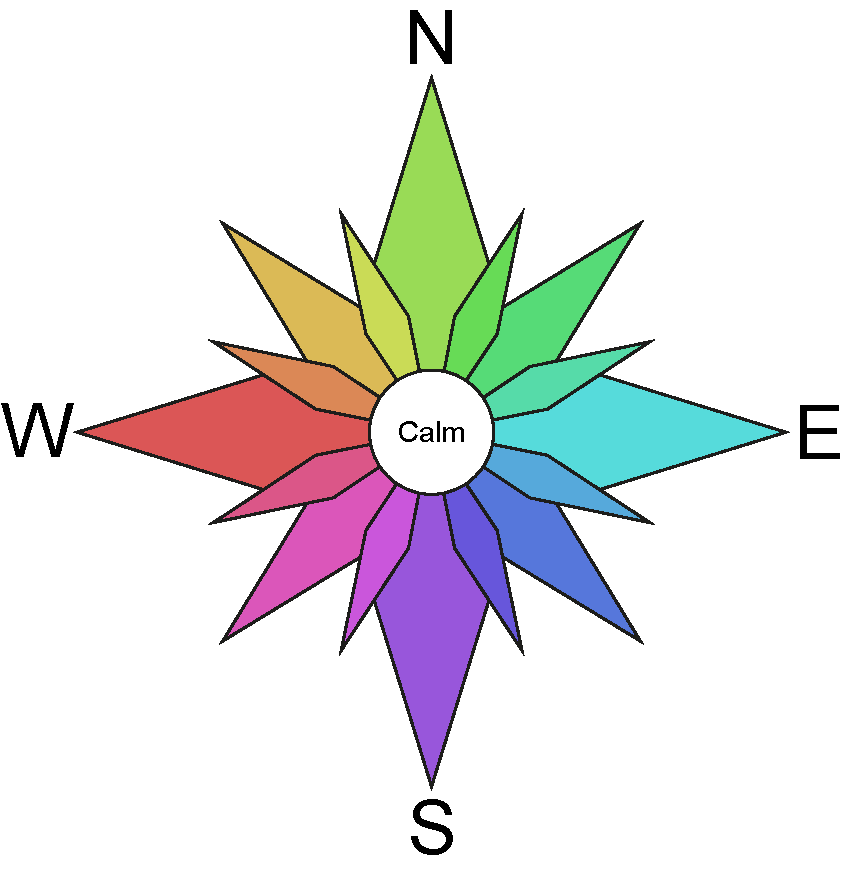
\includegraphics[width=\linewidth]{compass-rose.pdf}
    \caption[Compass Rose mapping colour to wind direction]{
        This compass rose shows the mapping of hue to wind direction used
        for figures below.  Colours are equidistant in the HSL colour space.}
    \label{fig:compass-rose}
\end{wrapfigure}



\Cref{fig:galiwinku-observations,fig:milingimbi-observations}
show historical weather observations at Galiwinku and Milingimbi as a set of
heatmaps (panels, arranged vertically).  Each heatmap is a grid, with year
on the y-axis and day-of-year on the x-axis.  Each cell is then shaded
according to the value observed on that day; days without data are shaded
black.
%
Unlike the climographs above, these figures clearly show variation in timing
of seasonal onset between years.  This demonstrates that timeseries data
at daily resolution is required for investigation of Indigenous seasons.

~\\

\todo{write detailed walkthrough of how to read these figures!
This means a walkthrough and interpretation of one panel, with
references to another.}


\begin{figure}[p]
    \centering
    \includegraphics[width=\textwidth]{galiwinku/observations.pdf}
    \caption[Historical weather observations at Elcho Island]{
        Historical weather observations at Elcho Island.
        Each panel shows a single variable, with years on the y axis and day-of-year on the x.
        Note that each variable has a different seasonal pattern,
        and that seasonality changes from year to year.}
    \label{fig:galiwinku-observations}
\end{figure}
% Note - if possible, these figures should be on facing pages to allow easy comparison
\begin{figure}[p]
    \centering
    \includegraphics[width=\textwidth]{milingimbi/observations.pdf}
    \caption[Historical weather observations at Milingimbi Airport]{
        Historical weather observations at Milingimbi Airport.
        Each panel shows a single variable, with years on the y axis and day-of-year on the x.
        Note that each variable has a different seasonal pattern,
        and that seasonality changes from year to year.}
    \label{fig:milingimbi-observations}
\end{figure}




\section{Quantifying a Yolngu Calendar}

\Cref{tab:quant-seasons-summary} summarises typical timing and recognition
criteria for each season.  \Cref{fig:season-definitions-code} shows the
implementation of these conditions in Python3 code -- normalised later --
which create the time-series shown in
\Cref{fig:galiwinku-seasons,fig:milingimbi-seasons}.

\begin{table}[h]
    \centering
    \begin{tabular}{llllll}
        Season          &  Typical Months       &  Criteria to recognise                    \\
        Dhuludur        &  Oct, Nov, Dec        &  Cool at night, mixed wind, first rain    \\
        Barramirri      &  Dec, Jan, Feb        &  NW wind, heavy rain most days            \\
        Mayaltha        &  Feb, Mar             &  NW wind, approx weekly rain              \\
        Midawarr        &  Mar, Apr, May        &  NE to E wind, less rain, last storm      \\
        Dharrathamirri  &  May, Jun, Jul, Aug   &  No rain, consistent ESE-SSE wind         \\
        Rarrandharr     &  Sep, Oct             &  Hot days, low humidity
    \end{tabular}
    \caption[A quantifiable summary of the Yolngu seasons case study]{
        A quantifiable summary of the Yolngu seasons case study.}
    \label{tab:quant-seasons-summary}
\end{table}

\begin{figure}[h]
    \lstinputlisting[firstline=31, lastline=55, xleftmargin=0.1\textwidth]{../code/season.py}
    \centering
    \caption[Python code: definition of season indicies]{
        Code listing of variables and conditions used to detect seasons.
        \todo{update detection, expand description, keep eye on line range.}
        }
    \label{fig:season-definitions-code}
\end{figure}

To avoid bloating this section, only figures for the seasons at Galiwinku
(Ngayawili weather station) are included in the text.  Corresponding
figures for all other stations can be found in the electronic appendicies;
interpretation of the figures below includes descriptions and comparisons
where relevant.

\begin{wrapfigure}{R}{0.5\textwidth}
    \centering
    \includegraphics[width=\linewidth]{galiwinku/season-pie.pdf}
    \caption[Calculated season frequency, Galiwinku]{
        Proportion of days on which each season was observed at
        Galiwinku, over the period of available data.
        These colours are used for each season in all figures below.
        }
    \label{fig:galiwinku-season-counts}
\end{wrapfigure}

\Cref{fig:galiwinku-season-counts} shows the proportion of days on which
each season was detected.  Like \cref{fig:compass-rose}, it also
shows a repeated colour scheme -- all season figures below use the
same colour palete, without further labelling.

~\\

\todo{Write interpretative para/s for index lines and observed area.}


\begin{figure}[h]
    \centering
    \includegraphics[width=0.8\textwidth]{galiwinku/seasons-daily-index.pdf}
    \caption[Season index by day-of-year, Elcho Island]{
        Mean normalised (z-score) index for seasons per day-of-year
        at Galiwinku.  Note the clear distinction in the dry season,
        but muddle in the Wet (Dec-Feb).
        This is not indicative of poor detection on a single day,
        but rather that occurence varies more between years.
        }
    \label{fig:season-daily-index}
\end{figure}
%
\begin{figure}[h]
    \centering
    \includegraphics[width=0.8\textwidth]{galiwinku/seasons-daily-prob.pdf}
    \caption[Season probability by day-of-year, Elcho Island]{
        Observed probability of each season by day of year.
        This figure does not show consistently strong ordering among all
        seseasons; this may be attributed to a combination of imperfect
        detection, true variation in seasonal occurance, and details
        lost in aggregation.
        }
    \label{fig:season-daily-prob}
\end{figure}


\todo{write paragraph/s interpreting multipanel season figs}


\begin{figure}[p]
    \centering
    \includegraphics[width=\textwidth]{galiwinku/seasons.pdf}
    \caption[Detected seasons for Elcho Island]{
        Detected seasons at Elcho Island, based on hand-crafted threshold conditions.
        DRAFT FIGURE ONLY, will change substantially as method improves.
        }
    \label{fig:galiwinku-seasons}
\end{figure}
% Note - if possible, these figures should be on facing pages to allow easy comparison
\begin{figure}[p]
    \centering
    \includegraphics[width=\textwidth]{milingimbi/seasons.pdf}
    \caption[Detected seasons for Milingimbi Airport]{
        Detected seasons at Milingimbi Airport, based on hand-crafted threshold conditions.
        DRAFT FIGURE ONLY, will change substantially as method improves.
        }
    \label{fig:milingimbi-seasons}
\end{figure}


\todo{Close section by summarising how well season detection worked.
Keep this impartial enough to fit results, rather than discussion.}



\section{Correlations with Climatic Indicies}
\label{sec:indicies-correlations}

\todo{analyse correlations between seasons and ENSO index/indicies, IOD, etc.}


